
\chapter{Estado de Arte}
\label{chapter:Estado de Arte}

\begin{Estado de Arte}

Neste capítulo será realizado um breve estudo teórico que permitirá uma melhor compreensão relativamente a conceitos que aqui serão abordados.

\end{Estado de Arte}

\section{Caixa de Velocidade}
Como o objetivo final desta dissertação é a classificação de uma caixa de velocidades como sendo defeituosa ou não, será necessário começar por explicar como é que esta funciona. Esta secção tem como base \textcite{formacaoCaixa}.

Todos os veículos automóveis necessitam de uma caixa de velocidades que permita, consoante a necessidade, converter o binário\footnote{Medida da força rotacional exercida sobre um eixo.} e a rotação do motor para as rodas.
Se o motor do veículo fosse ligado diretamente às rodas, com uma relação de transmissão fixa, verificar-se-ia que o binário por este disponibilizado seria manifestamente insuficiente para proceder ao arranque do veículo ou, então, que a velocidade máxima do veículo seria extremamente baixa.

De uma forma geral e simplificada, quanto maior a rotação do motor em relação à rotação do eixo das rodas, maior será o binário e, quanto menor a rotação do motor em relação à rotação do eixo das rodas, maior será a velocidade. Normalmente esta proporção expressa-se tecnicamente por 10:1, 9:1, 1:1.05, 1:7 e assim por diante.

\subsection{Constituição}

Como os automóveis franceses são maioritariamente automóveis a tração com um motor transversal estes usam, portanto, ``caixas-ponte''.
Estas caixas são constituídas principalmente por 4 órgãos (fig. \ref{caixa_velocidades}) : o cárter, as árvores, os comandos internos e o diferencial (ou ponte).

\begin{figure}[H]
\centering
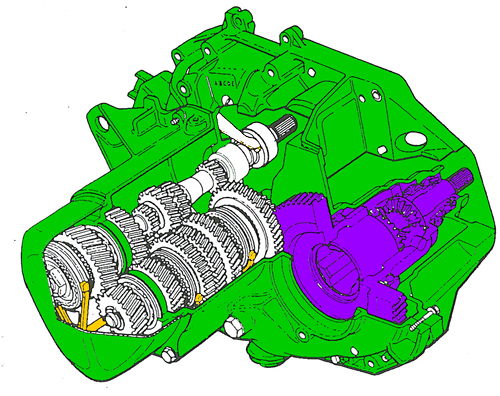
\includegraphics[scale=1.0]{figs/caixa}
\caption{Caixa velocidades e seus órgãos: cárter(verde), carretos(branco), comandos internos(amarelo), diferencial(roxo)}\label{caixa_velocidades}
\end{figure}

O cárter têm 3 funções: proteger os carretos da caixa de velocidade, criar um espaço impermeável para poder lubrificar os carretos e resistir às forças de engrenamento nos apoios dos rolamentos. A lubrificação é um ponto crucial numa caixa de velocidades pois permite reduzir a fricção, isto é, o desgaste das peças. Também permite evitar a gripagem\footnote{Efeito produzido pela fricção de duas superfícies metálicas em contacto, e que, por falta de uma lubrificação suficiente, aderem uma à outra.} das peças em movimento.

As árvores (fig. \ref{carreto}) são um conjunto composto principalmente por várias engrenagens, pinhões, anéis e anéis de arrasto. O par de engrenagens permite obter velocidades de rotação e binários diferentes em função da velocidade selecionada. A roda que provoca o efeito de rotação (roda de entrada de movimento) é chamada de mandante e a roda que sofre o efeito (roda de saída de movimento) é chamada de mandada. A relação de transmissão é dada pelo número de dentes da roda mandada a dividir pelo número de dentes da roda mandante. Quanto maior for a relação de transmissão maior é a velocidade de rotação da roda mandada e mais fraco o seu binário. Quantos mais dentes tem a roda dentada mandada relativamente à roda mandante menor é a sua velocidade de rotação, mas o binário do conjunto aumenta. Aplicando este conceito a uma caixa de velocidades, onde existem dois eixos: a árvore primária, que recebe do volante do motor a rotação do motor por intermédio da embraiagem e por isso onde se encontram as rodas mandantes, e a árvore secundária, que transmite um submúltiplo dessa rotação ao diferencial\footnote{O diferencial tem a função de distribuir o binário a dois semi-eixos que por sua vez estão ligados às rodas.}. Será importante frisar que os carretos da árvore secundária se encontram em rotação livre, o que permite que, em ponto morto (ex., sem nenhuma velocidade engrenada), não ocorra a transferência de movimento.
Mudar de mudança significa mudar a relação de transmissão, quanto maior for a mudança menor será a relação de transmissão deste modo mais baixo é o binário disponível e maior é a velocidade à saída. Em situações que seja preciso inverter o sentido de marcha(marcha-atrás), como não é possível inverter o sentido de rotação do motor, é intercalado um carreto adicional entre a roda mandante e mandada, invertendo assim o sentido de rotação da roda mandada final.

\begin{figure}[H]
\centering
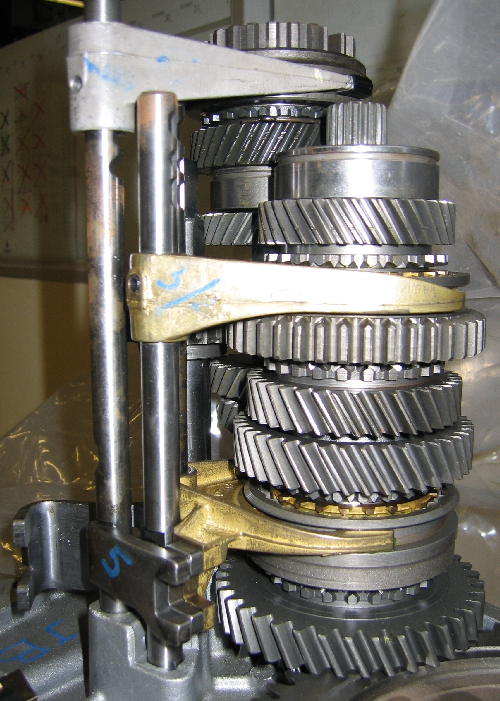
\includegraphics[scale=1.0]{figs/carretos}
\caption{Carreto}\label{carreto}
\end{figure}

O comando interno (fig. \ref{comando interno}) é o que permite fazer a seleção de velocidade, é um conjunto de peças que é acionado pelo condutor com ajuda da alavanca de mudanças, quando o veículo se encontra em deslocamento. O eixo secundário, para cada velocidade, tem um carreto louco que é capaz de girar livremente à volta do eixo secundário e está engrenado com um carreto fixo do eixo primário. O movimento da alavanca de mudanças vai levar à deslocação de eixos/forquilhas que estão diretamente engatados no anel de arrasto e que por sua vez provocará a transferência do anel de arrasto. Este anel é responsável por transmitir o movimento de rotação do carreto louco até ao eixo secundário. Como o carreto louco e o anel de arrasto não têm a mesma velocidade de rotação, para evitar qualquer risco de rutura, sincronizam-se as velocidades de rotação antes do engrenamento. Isto é feito utilizando um sincronizador, que com o atrito, ao encostar ao carreto as rotações são sincronizadas.

\begin{figure}[H]
\centering
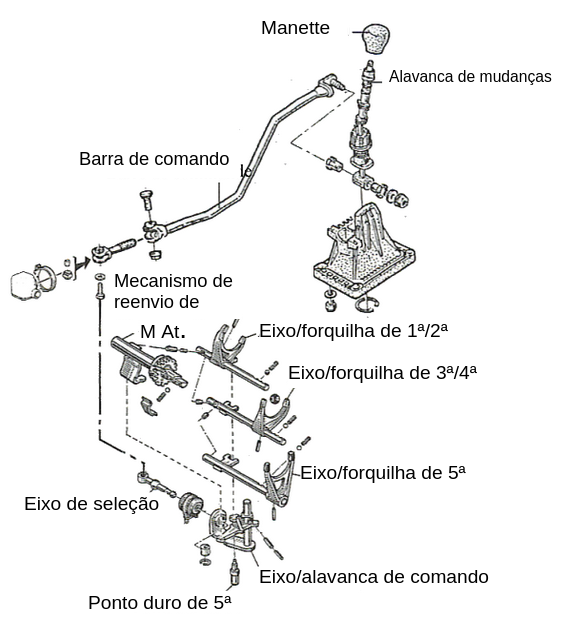
\includegraphics[scale=0.4]{figs/comando_interno}
\caption{comando interno}\label{comando interno}
\end{figure}

O diferencial serve para que numa curva, como a roda exterior percorre uma maior distância do que a roda interior, a velocidade de rotação da roda exterior é maior do que a roda interior. O diferencial permite, nas curvas, distribuir a potência a cada roda, podendo inclusive uma roda permanecer em repouso enquanto a outra recebe toda a potência e movimento gerado pelo motor. Isto acontece porque a força tende a “ seguir o caminho mais fácil ”.


\section{Acústica}

A experiência e o conforto que um condutor tem a conduzir um automóvel são fatores importantes, que são influenciados por uma combinação entre: ruído, vibrações e severidades sentidas no veículo. O NVH (\textit{``Noise,Vibration and Harshness''}) é o estudo e modificação dos ruídos e vibrações característicos dos veículos (principalmente carros e caminhões). Embora o ruído e as vibrações possam ser medidos, a ``severidade'' designa um aspeto subjetivo da acústica, mensurável por um júri acústico ou por instrumentação ``especial'' que reflete os sentimentos humanos: trata-se da psicoacústica.

A vibração traduz um movimento oscilante de um ponto de uma estrutura e o ruído reflete um movimento oscilante do ar. Geralmente distinguimos os 3 elementos seguintes: A fonte, que muitas vezes é vibratória, mas também pode ser diretamente acústica; o transmissor, que amplifica ou atenua o ruído; e o emissor, também denominado altifalante que neste caso pode ser os painéis, janelas ou pára-brisas por exemplo. No caso de um veículo em andamento os transmissores são: o ar diretamente, o ruído produzido pela corrente cinemática é propagado no ar até ao ouvido do condutor com a janela aberta, o ar indiretamente, o ruído é propagado e absorvido pelas janelas ou painéis atuando como emissores, e por fim por via sólida, as vibrações propagam-se na carroçaria e vibram nos subconjuntos (porta traseira, chão). Por vezes identificar a fonte poderá ser complicado pois o transmissor e o emissor podem cada um  modificar o tom original do ruído \cite{bruitChaine}. 
\subsection{As diferentes fontes de som de uma caixa de velocidades}
Segundo \textcite{Grainolement}, a principal fonte de ruído em um veículo é o motor e a caixa de velocidades. Numerosos estudos e soluções foram realizados no que diz respeito ao motor em termos de suas emissões de ruído. Mas a redução no ruído do motor destaca evidência dos ruídos produzidos pela caixa de velocidade. As vibrações são transmitidas para a caixa de velocidades de duas maneiras:
\begin{itemize}
\item Via sólida: as vibrações que aparecem ao nível das engrenagens são
transmitidas para as árvores, em seguida, para os rolamentos e para o cárter;
\item Via aérea: dentro do cárter, as vibrações dos elementos mecânicos criam
diferenças de pressão; sob o efeito dessas tensões, a estrutura da caixa
comporta-se quase como a membrana de um altifalante(emissor): a caixa ``irradia''.
\end{itemize}
As fontes de ruído numa caixa de velocidade são:
\begin{itemize}
\item árvores devido a defeitos de coaxialidade e cilindricidade\footnote{Cilindricidade é uma tolerância tridimensional que controla a forma geral de um recurso cilíndrico para garantir que seja redondo e reto o suficiente ao longo de seu eixo.},
\item rolamentos devido à folga, defeitos de desgaste,
\item as engrenagens.
\end{itemize}

Engrenagens são a principal causa de ruído na caixa de engrenagens devido aos contactos perpétuos existente entre os dentes das engrenagens engatadas ou livres. A sua geometria é, portanto, otimizada para reduzir o ruído de engrenamento tanto quanto possível. No entanto falhas podem ocorrer como:
\begin{itemize}
\item defeito de fabrico: espaçamento irregular entre os dentes, pinhões não totalmente circulares,
\item amplificação de vibrações em frequências correspondentes às características modais
do sistema: modos de flexão ou torção dos dentes, eixos, etc.,
\item efeito de sucção: bolsas de ar ou óleo formadas durante o desengate de um dente.\cite{Grainolement}
\end{itemize}

Inicialmente todas as caixas eram feitas com dentado reto (fig. \ref{dentado_reto}), mas por uma questão acústica passaram a ser dentado helicoidal (fig. \ref{dentado_helicoidal}) por este permitir um escorregamento entre dentes que por sua vez diminui o ruído de contacto individual de cada dente. A engrenagem helicoidal permite que 2 pares de dentes estejam em contacto em simultâneo. 

\begin{figure}[H]
\centering
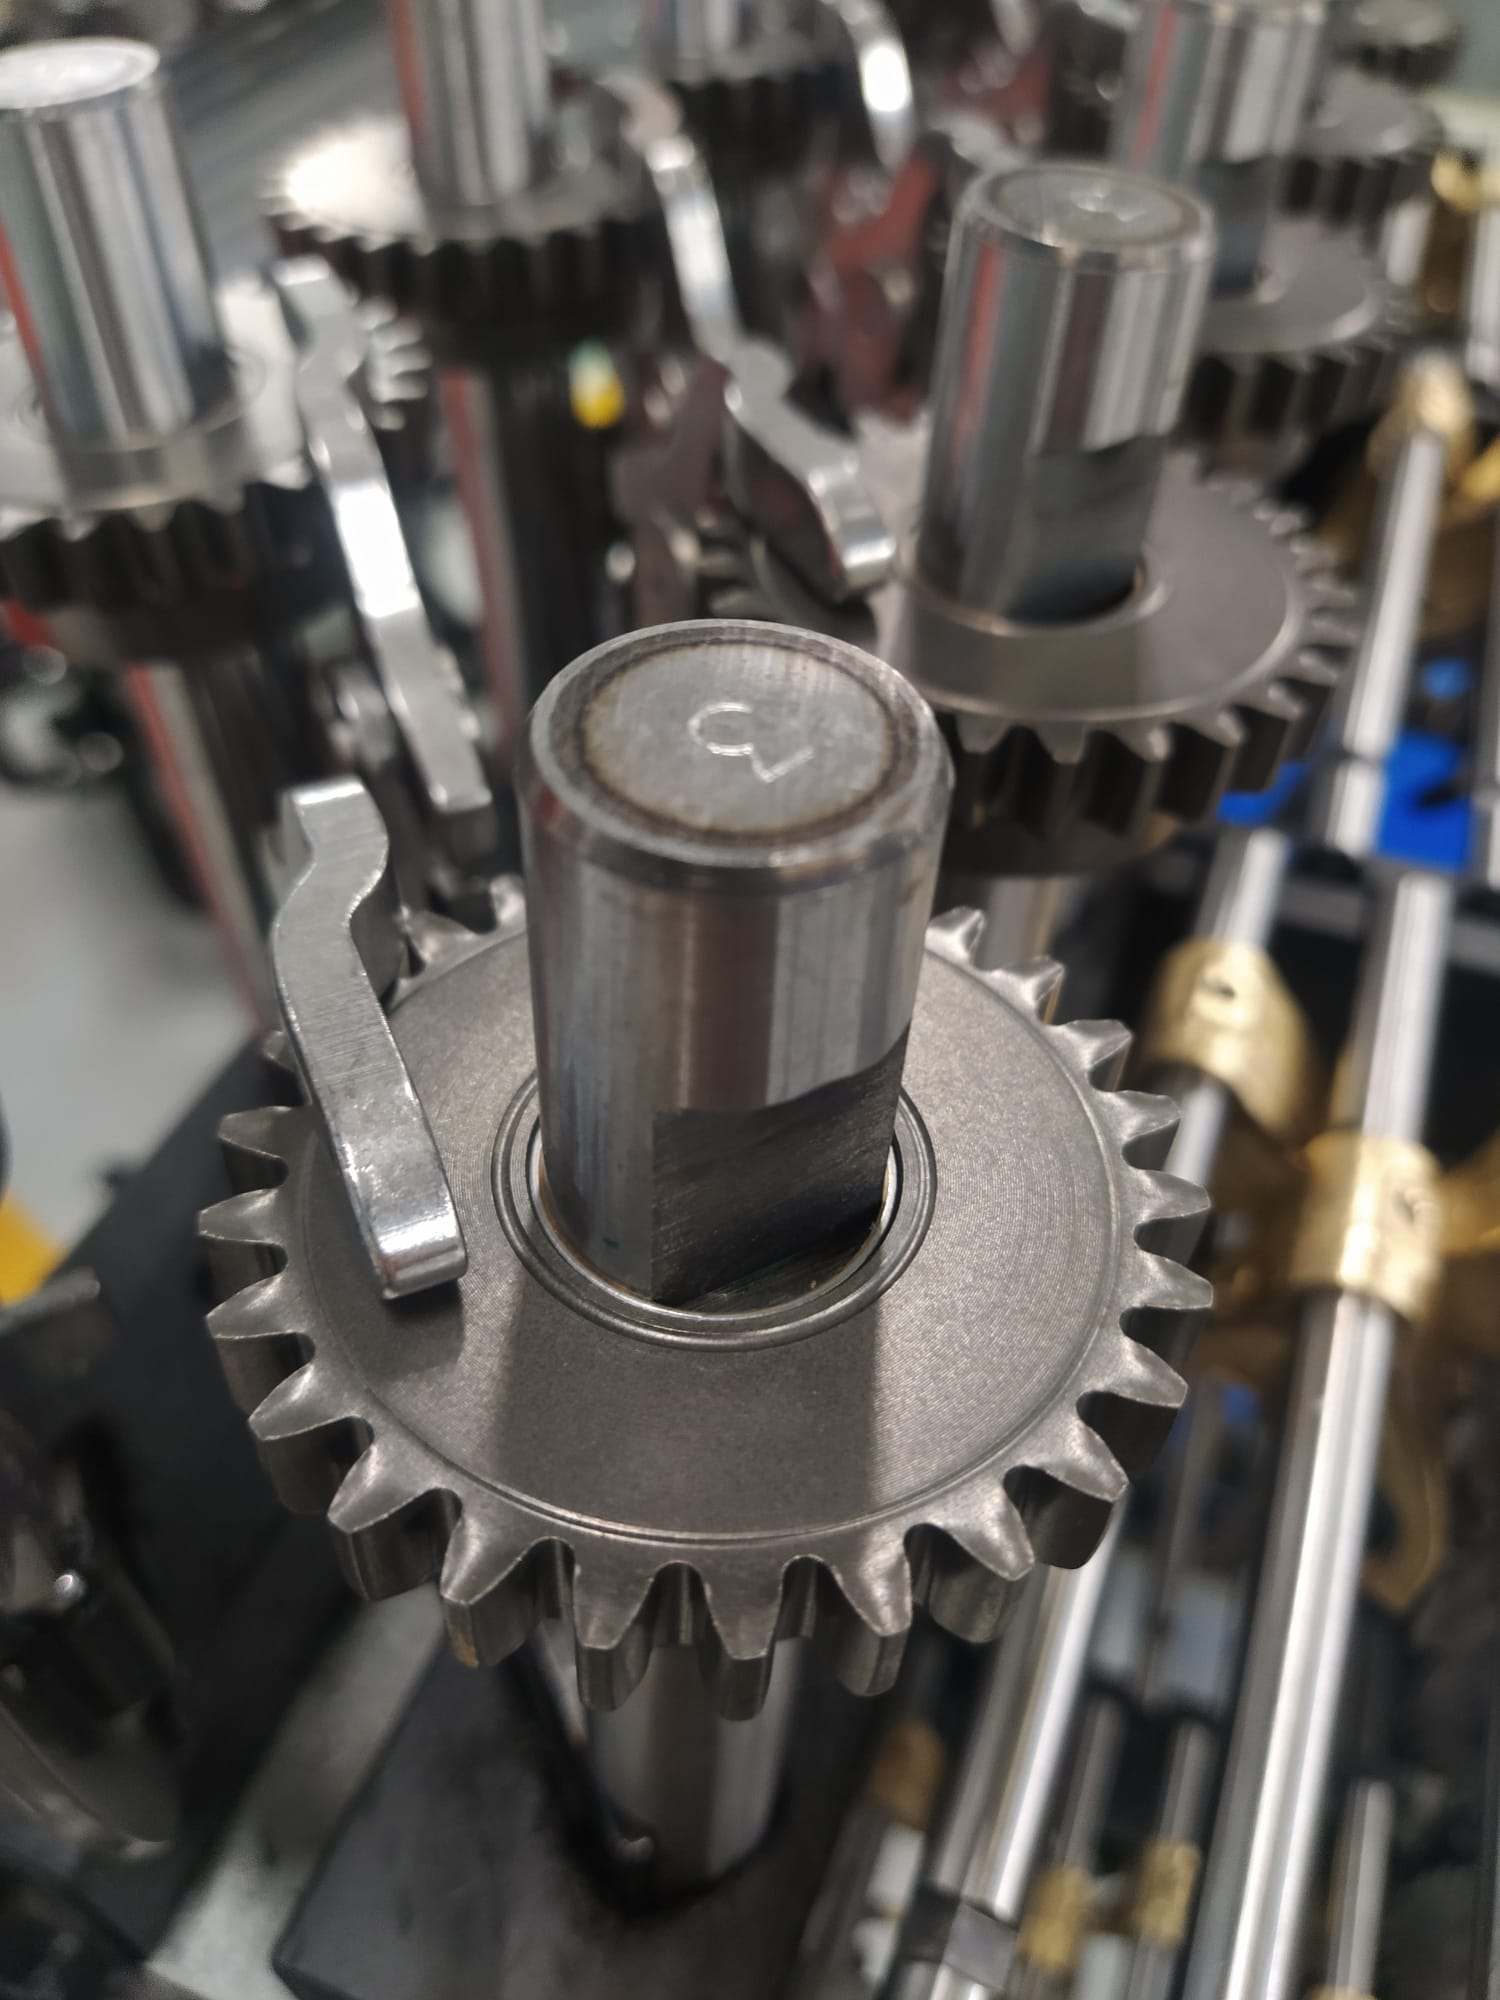
\includegraphics[scale=0.1]{figs/dentado_reto}
\caption{Engrenagem com dentado reto}\label{dentado_reto}
\end{figure}



\begin{figure}[H]
\centering
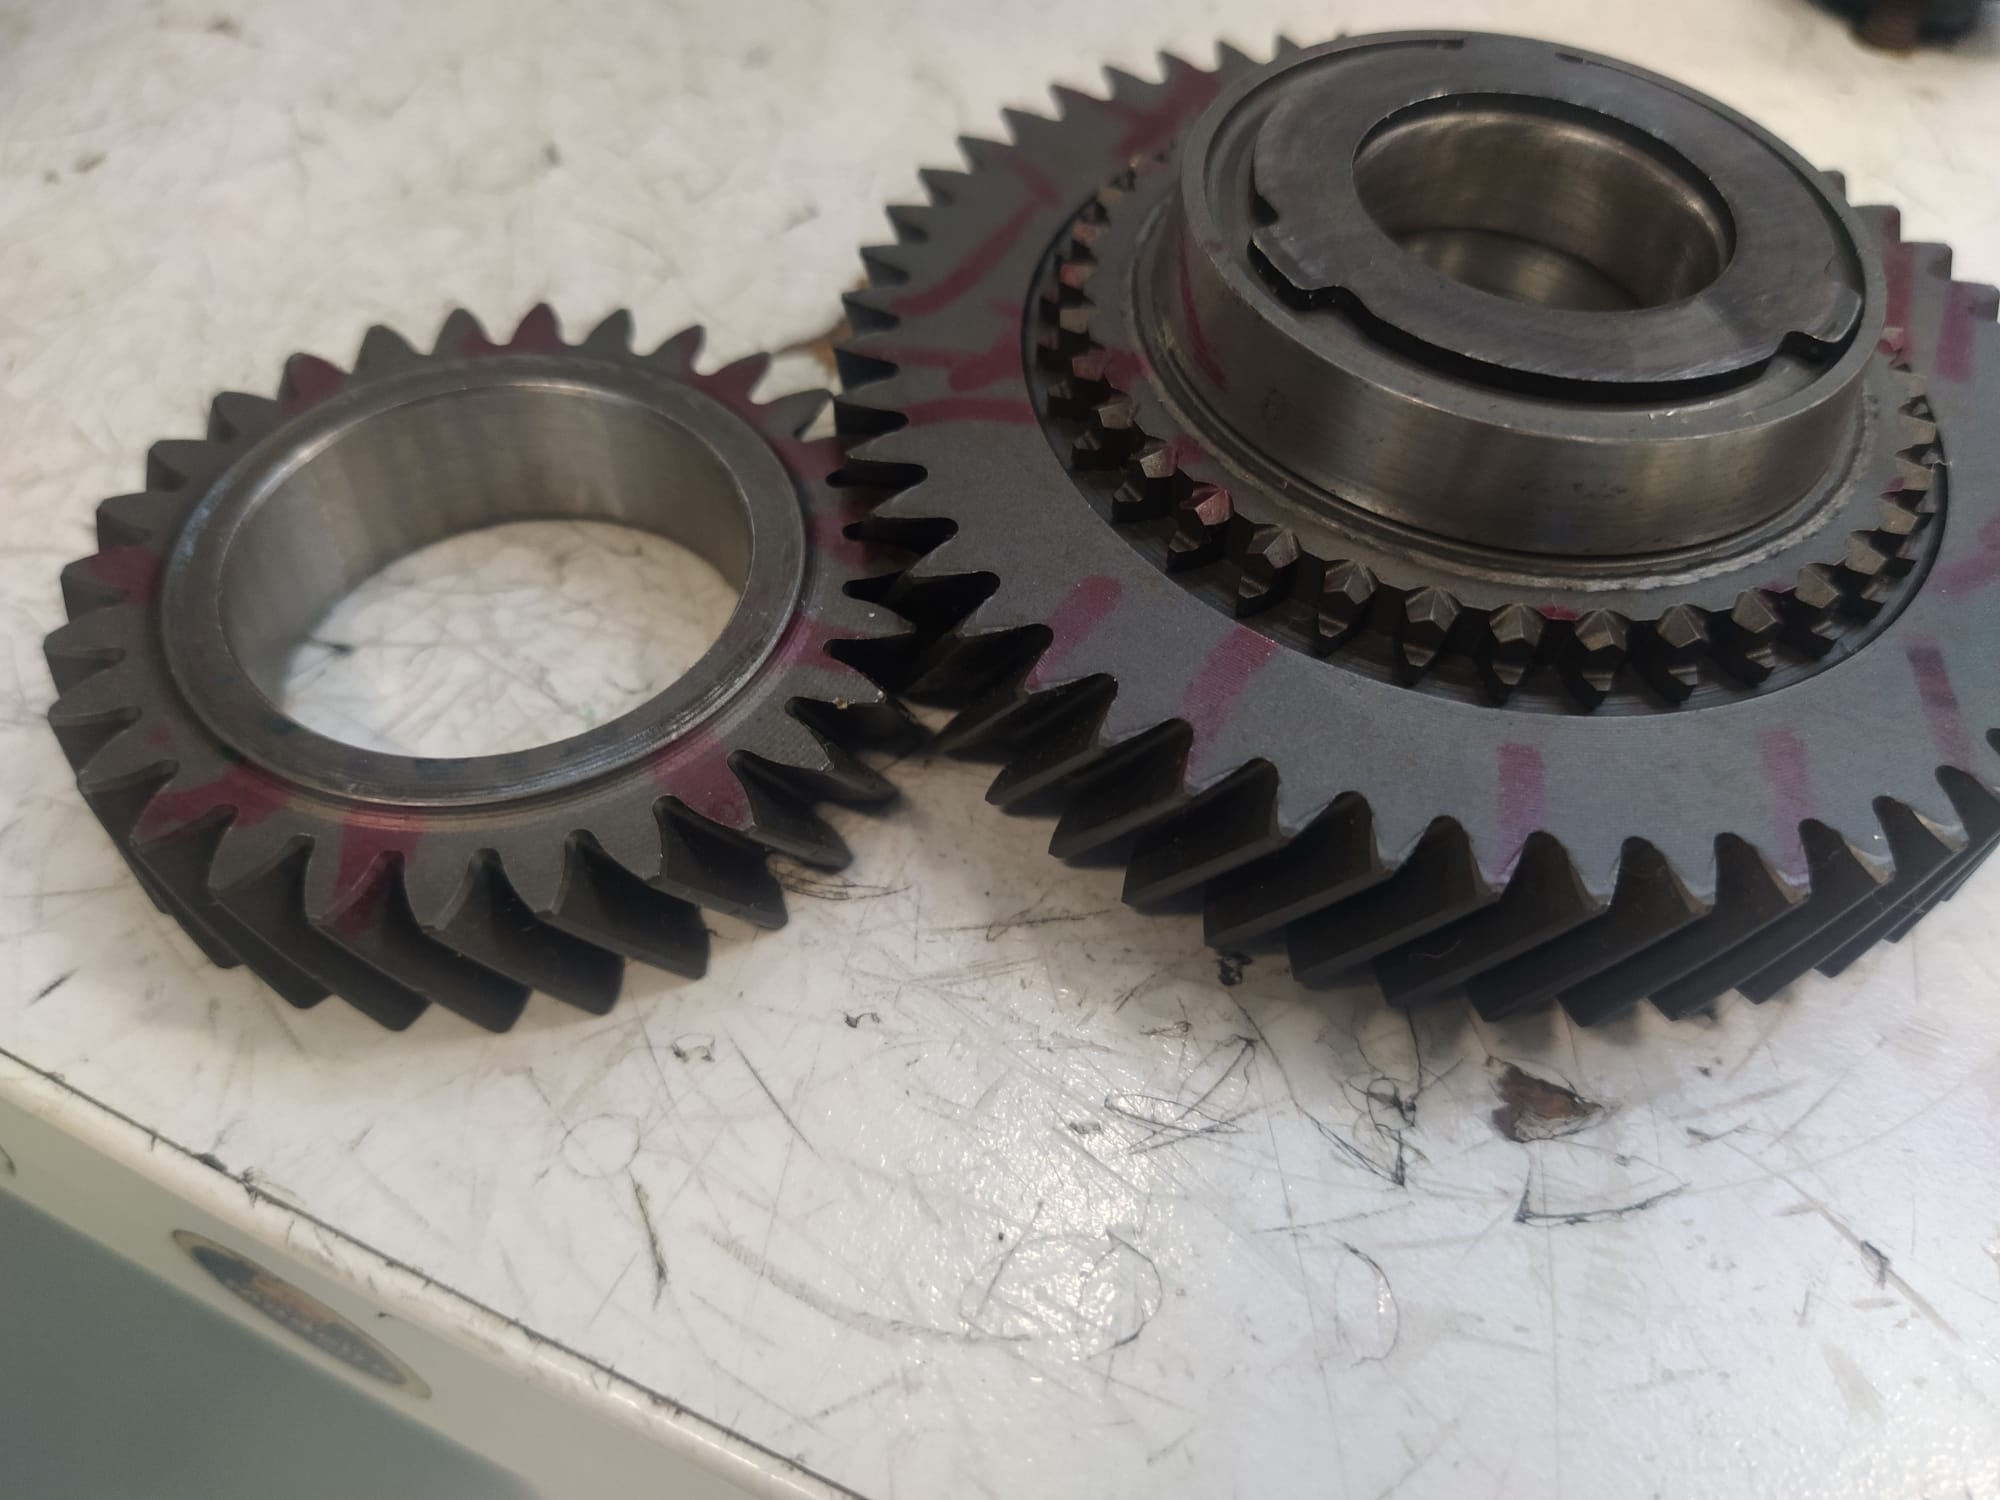
\includegraphics[scale=0.1]{figs/dentado_heli}
\caption{Engrenagem com dentado helicoidal}\label{dentado_helicoidal}
\end{figure}


\section{analise vibratória}
As caixas de velocidade são usadas em diferentes condições: velocidades altas e/ou cargas altas. Qualquer pequena falha em um componente da caixa de velocidades pode originar uma falha ou ruídos inesperados. Como as caixas de velocidade têm uma estrutura complexa, conseguir detetar e prever defeitos na fase de montagem terá o beneficio de reduzir dano consequencial, aumentar a vida útil da caixa, reduzir o armazenamento de peças sobressalentes, reduzir a manutenção de avarias e evitar uma perda de tempo e dinheiro. Para uma deteção precoce é feita uma analise ao sinal vibratório. A Renault Cacia utiliza diversos métodos de análise que irão ser descritos aqui.


\subsection{Análise em frequência}
A análise em frequência é o método mais usado para analisar sinais vibratórios. O tipo mais básico desta analise é uma FFT ou ``Fast Fourier Transform'' que converte um sinal do domínio do tempo para o domínio da frequência. O produto desta conversão é um espectro de potência (ou energia) que mostra a energia contida em frequências específicas do sinal em geral.

Apesar do seu uso comum, existem várias contras em só usar a análise em frequência devido aos seus resultados, como o espectro de potência ou distorção harmónica total, conter apenas a informação de todo o sinal distribuída pelas várias frequências. Não contém informação temporal. Isto implica que a análise em frequência não é adequada para sinais no qual as frequências de certos componentes variam ao longo de tempo.
\subsection{Análise de ordem}
A análise de ordem é a arte e a ciência de extrair conteúdos sinusoidais de medições de sistemas acústico-mecânicos sob carregamento periódico. A caraterística principal é de a medição estar relacionada com as revoluções, a velocidade de rotação e as ordens harmónicas das partes rotativas. Usada principalmente para encontrar soluções para problemas, no design e para testar produtos, que é o nosso caso. A chave para a análise de ordem é a informação sobre a velocidade de rotação, que é obtida através de um taquímetro (fig. \ref{taquimetro}).

\begin{figure}[H]
\centering
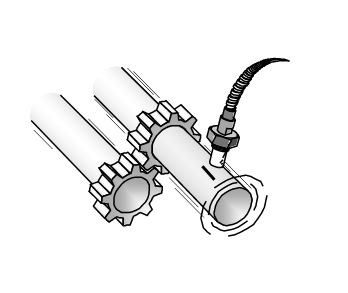
\includegraphics[scale=0.5]{figs/tacho_signal}
\caption{Taquímetro}\cite{orderAnalysis}\label{taquimetro}
\end{figure}

Com base no exemplo dado em \cite{orderAnalysis2} e para melhor entender a análise de ordem a figura (fig. \ref{power espectrum 1})  contém um espectro de potência. Existem dois picos, o primeiro a 60Hz corresponde à velocidade de rotação do eixo de uma máquina, e o  segundo pico, que é o 4º harmónico da velocidade de rotação, corresponde aos rolamentos da máquina. Se pretendermos monitorizar a saúde dos rolamentos é importante seguirmos este 4º harmónico.

\begin{figure}[H]
\centering
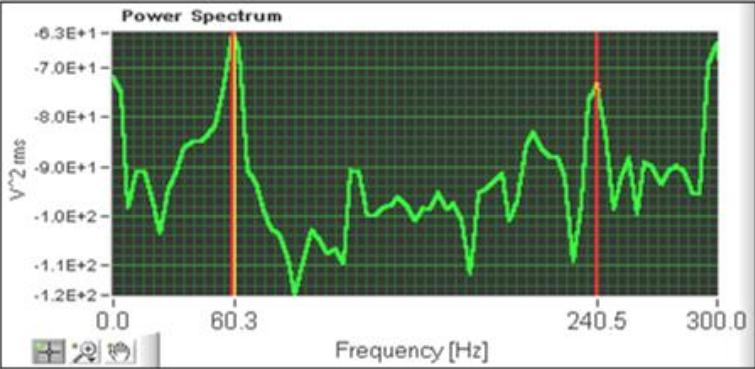
\includegraphics[scale=0.3]{figs/power_spectrum1}
\caption{Espectro de potência de uma caixa de velocidades de uma eólica a 60Hz}\label{power espectrum 1}
\end{figure}


No entanto, à medida que a velocidade diminui para 50Hz, o 4º harmónico do espectro de potência desloca-se. Os picos num espectro de potência de um componente rotativo estão todos relacionados à velocidade rotação  fundamental desse componente. Mesmo que o FFT seja capaz de analisar os dados e mostrar o espectro de potência, não é capaz de facilmente monitorizar os harmónicos (fig. \ref{power espectrum 2}).

\begin{figure}[H]
\centering
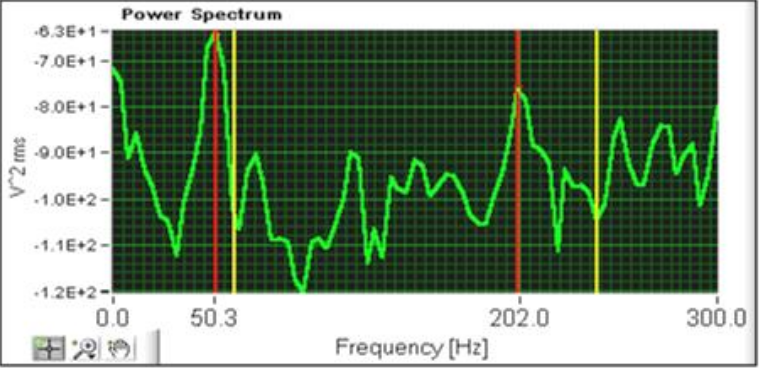
\includegraphics[scale=0.3]{figs/power_spectrum2}
\caption{Espectro de potência de uma caixa de velocidades de uma eólica a 50Hz}\label{power espectrum 2}
\end{figure}

Na análise de ordem o sinal é primeiro reamostrado no domínio angular. A reamostragem combina as medições de velocidade tiradas de um taquímetro na máquina com as medições de vibração e interpola as medições de vibração em um ponto de dados por fração de rotação angular. As medições de vibração estão agora no domínio angular em vez de estarem no domínio de tempo. Uma vez no domínio angular uma FFT pode ser realizada nas medições de vibração para obter o que é conhecido por um espectro de ordem.


\begin{figure}[H]
\centering
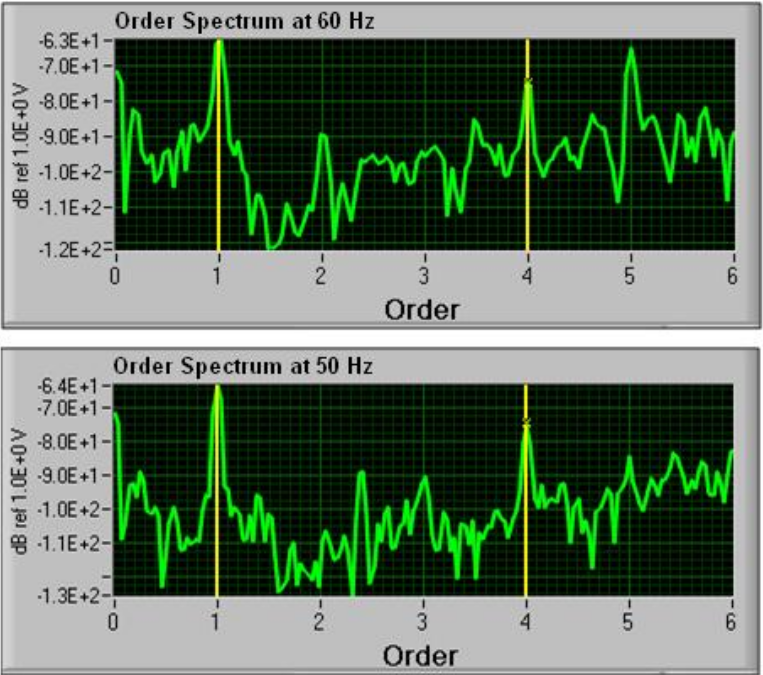
\includegraphics[scale=0.3]{figs/order_spectrum}
\caption{Espectro de ordem de uma caixa de velocidades de uma eólica a 60Hz(topo) e 50Hz(fundo)}\label{power espectrum 3}
\end{figure}


Com o espectro de ordem torna-se mais fácil monitorizar o 4º harmónico pois este não se desloca conforme a velocidade de rotação aumenta ou diminui. Ordem 1 corresponde a 1x a velocidade de rotação, todas as outras ordens são múltiplas da primeira, sendo que ordem 4 corresponde a 4x a velocidade de rotação.

\subsection{Cepstrum}

A análise de Cepstrum tem diversas aplicações, como na deteção e remoção de eco ou na análise da fala. Uma das mais importante está relacionada com industria, no diagnóstico de máquinas, onde a sua habilidade para detetar periodicidades no espectro é aproveitada.

O espectro de uma caixa de velocidades é usualmente constituído por um número de famílias de harmónicos. Estas famílias de harmónicos são originadas pelos eixos rolamentos e pelas frequências dos dentes engrenados das engrenagens. É comum as engrenagens terem um número ímpar de dentes, isto é uma vantagem pois faz com que o desgaste se espalhe uniformemente, mas também é uma vantagem no ponto de vista de medição já que as diferentes famílias de harmónicos não se vão sobrepor. Por outro lado, muitas das vezes pode haver várias famílias de harmónicos, o que pode ser difícil para poder separá-las no espectro. O Cepstrum é uma ferramenta prática que permite facilmente encontrar as diferentes famílias de harmónicos, nas quais podem ser monitorizadas individualmente para procurar alterações que poderão ser um indicador de que algo está errado\cite{Notes2}.

O Cepstrum, como pode ser visto em \textcite{Notes}, é definido como o ``inverso da transformada de Fourier do espectro de potência logarítmico'': 

\begin{equation}
	C_{xx} = \mathcal{F}^{-1} \left \{ \log F_{xx}\left ( f \right ) \right \}
\end{equation}

	
	onde $F_{xx}$ é o espectro de potência. O Cepstrum e a auto-correlação estão fortemente relacionados. A auto-correlação pode ser obtida fazendo o inverso da transformada de Fourier do espectro de potência: 
	
\begin{equation}
	R_{xx} = \mathcal{F}^{-1} \left \{ F_{xx}\left ( f \right ) \right \}
\end{equation}


A auto-correlação é principalmente dominada pelos maiores valores do espectro. O logaritmo usado no cálculo do Cepstum faz com que ele tenha mais em conta os harmónicos de baixo nível em comparação com a auto-correlação. Também significa que a auto-correlação é fortemente influenciada pela forma do sinal no tempo enquanto que no Cepstrum reage principalmente aos harmónicos presentes no espectro e não tanto aos seus tamanhos relativos.

Segue-se um exemplo para demonstrar a capacidade do Cepstrum como ferramenta para medições. A figura \ref{spectrum Cepstrum1} representa o espectro de potência do sinal vibratório de uma caixa de velocidades de apenas uma velocidade. Ao analisar o espectro, encontramos uma ``floresta'' de harmónicos. Se quisermos encontrar uma família de harmónicos teríamos de o fazer manualmente o que é um processo tedioso.
	

\begin{figure}[H]
\centering
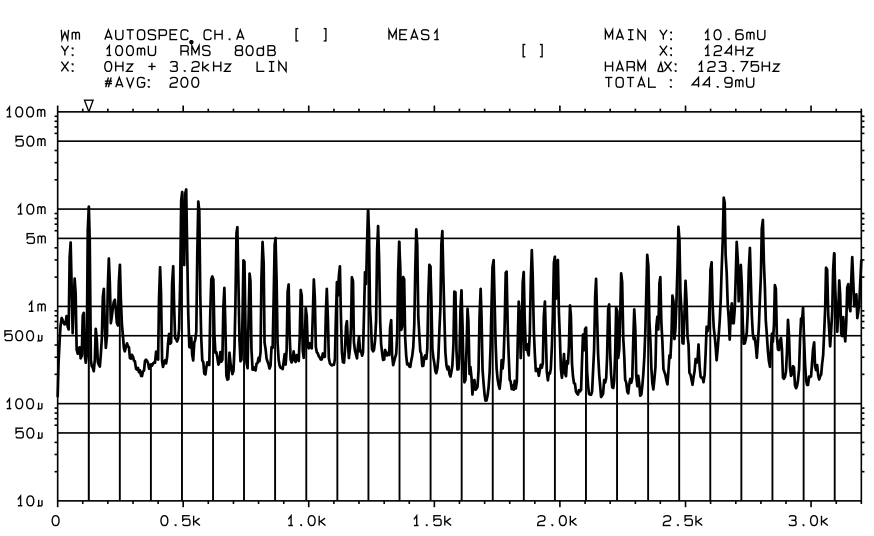
\includegraphics[scale=0.35]{figs/spectrum_cepstrum1}
\caption{Espectro de potência do sinal vibratório de uma caixa de velocidades (1 velocidade)}\label{spectrum Cepstrum1}
\end{figure}


O processo de encontrar as famílias de harmónicos é muito mais fácil no domínio do Cepstrum (fig \ref{spectrum Cepstrum2}). Como podemos observar neste caso encontramos duas famílias de harmónicos, uma representada pela letra A e outra pela letra B.


\begin{figure}[H]
\centering
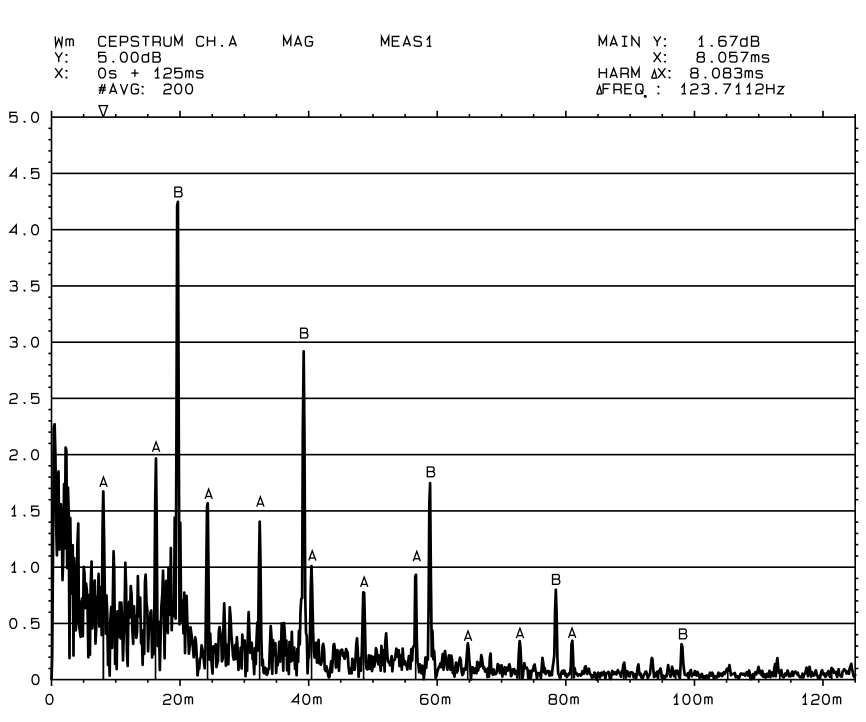
\includegraphics[scale=0.35]{figs/spectrum_cepstrum2}
\caption{Cepstrum do sinal vibratório de uma caixa de velocidades (1 velocidade)}\label{spectrum Cepstrum2}
\end{figure}

\subsection{Kurtosis}

Outra métrica de bastante utilidade no diagnóstico de problemas numa caixa de velocidade é a Kurtosis, apresentada em \cite{Kurtosis}. Sinais com o valor de Kurtosis maior têm mais picos que são maiores que 3x o valor quadrático médio (RMS) do sinal.

A Kurtosis pode ser expressa como o valor normalizado ``K''. A expressão\ref{expressao1} seguinte mostra o cálculo de K para N amostras.


\begin{equation}	
	K = \frac{\frac{1}{n}\sum \left ( x_{i}^{4} \right )}{(\frac{1}{n}\sum (x_{i}^{4}))^{2}}
\label{expressao1}
\end{equation}

No gráfico seguinte (fig \ref{kurtosis1}) podem ser vistos dois sinais, um sinal Gaussiano puro, que tem sempre K = 3, e um sinal com K = 4. O sinal com maior valor de kurtosis passa mais tempo em amplitudes maiores.

%acrecentar foto do outro grafico com ume xemplo real

\begin{figure}[H]
\centering
\includegraphics[scale=0.3]{figs/Kurtosis1}
\caption{Comparação entre um sinal Gaussiano com K = 3 e um sinal com k = 4 }\label{kurtosis1}
\end{figure}

Caso uma caixa de velocidade tenha uma engrenagem com um defeito num dente, no espectro de potência irá surgir um pico de maior intensidade. O valor da kurtosis para esta caixa será superior em relação ao valor da kurtosis de uma outra caixa em boas condições.


%picos fora do normal, quao itensos sao relativamente a media

%O ultrassom permite destacar os harmónicos motores, as ressonâncias das estruturas e também os fenómenos de choques.
%O harmónico corresponde a uma excitação que ocorre n vezes por revolução da cambota para uma determinada mudança e a sua frequência é %dada por: $f_{Hn}^{N}=n\frac{N}{60}$ , onde N representa os rpm  e Hn a ordem do harmónico. Num motor a 4 tempos o harmónico H2 (ordem %2) é o mais energético devido ao facto de haver 2 explosões por rotação da cambota.



\section{Machine Learning}

Inteligência Artificial (\ac{ia}) é definida como o estudo de agentes inteligentes, que podem perceber o ambiente e agir de forma inteligente da mesma forma que os humanos.
Machine Learning (\ac{ml}\footnote{Aprendizagem automática em português.}) é um sub-campo de \ac{ia} e envolve o estudo científico de modelos estatísticos e algoritmos que conseguem aprender progressivamente com os dados e atingir uma performance desejada.
Isto faz com que \ac{ml} possa ser usada em diversas tarefas que necessitem de automação e especialmente em cenários onde os humanos não podem desenvolver manualmente um conjunto de instruções para automatizar as tarefas desejadas. 

Já que os termos \ac{ml} e Deep Learning (\ac{dl}\footnote{Aprendizagem profunda em português.}) tendem a ser confundidos, é importante observar as nuances entre os dois. Redes neurais, \ac{ml} e \ac{dl} são todos sub-campos de \ac{ia}. No entanto, \ac{dl} é um sub-campo de \ac{ml} e rede neural um sub-campo de \ac{dl}\ref{relation}. A diferença entre \ac{dl} e \ac{ml} está na forma de como cada algoritmo aprende. Em \ac{dl}, a maior parte do processo de extração de caraterísticas (``Feature extraction'')\footnote{Processo que envolve simplificar o conjunto de dados requeridos para descrever um grande conjunto com mais precisão.} é automatizado, eliminando assim alguma da intervenção manual humana necessária e possibilitando o uso de conjunto de dados maiores. \cite{MLIBM}




\begin{figure}[H]
\centering
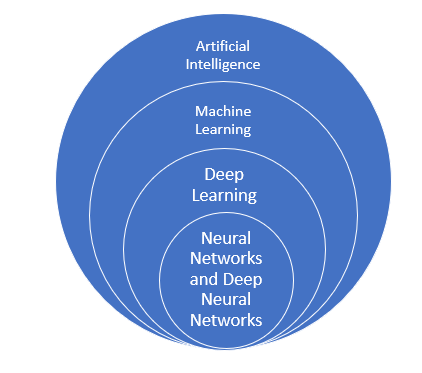
\includegraphics[scale=0.6]{figs/ai_relationship}
\caption{Relação entre \ac{ia}, \ac{ml} e \ac{dl} }\cite{imagemRelation}\label{relation}
\end{figure}



Geralmente um algoritmo de machine learning consiste aproximadamente em 3 componentes:

\begin{itemize}
\item \textbf{Um processo de decisão}: Os algoritmos de \ac{ml} são usados para fazer uma previsão ou classificação. Com base em alguns dados de entrada o algoritmo vai produzir uma estimativa sobre um padrão nesses dados.
\item \textbf{Uma função de erro}: serve para avaliar a previsão do modelo. Se existem exemplos conhecidos, a função de erro pode fazer uma comparação para averiguar a exatidão do modelo.
\item \textbf{Um processo de otimização de modelo}: O algoritmo ajusta como o processo de decisão chega à decisão final, numa tentativa de reduzir as previsões erradas. O algoritmo irá repetir este processo de avaliação e otimização até que um determinado limite de exatidão é atingido.
\end{itemize}

Muitos modelos de \ac{ml} são definidos pela presença ou não de influência humana sobre os dados, e  enquadram-se nas seguintes três categorias principais:
\begin{itemize}
\item \textbf{Aprendizagem supervisionada}:  é definida pelo uso de conjuntos de dados pré-rotulados (entradas e suas saídas desejadas) para treinar o algoritmo a encontrar uma regra geral que mapeie as entradas às saídas. À medida que os dados de entrada são alimentados no modelo, ele faz uma série de ajustes internos até que fique afinado corretamente. É usado em dois tipos de cenários: problemas de classificação, categorizar dados de teste; e problemas de regressão, perceber a relação entre variáveis dependentes e independentes.


\item \textbf{Aprendizagem não supervisionada}: o algoritmo recebe um conjunto de dados não rotulado, isto é, apenas com entradas, e encontra uma estrutura nos dados, como padrões e agrupamentos. Não existe intervenção humana no conjunto de dados fornecido ao algoritmo mas existe na validação das variáveis de saída (verificar se as conclusões tiradas pelo algoritmo são desejadas).


\item \textbf{Aprendizagem semi-supervisionada}: um meio termo entre aprendizagem supervisionada e não supervisionada. O conjunto de dados contém  dados estruturados e não estruturados, que irão guiar o algoritmo a tirar conclusões independentes. O uso dos dois tipos de dados num conjunto de dados para treino permite ao algoritmo de \ac{ml} aprender a rotular conjunto de dados não rotulados.

\end{itemize}

\subsection{Rede Neural Artificial}

Uma rede neural Artificial (ANN, Artificial Neural Network) é um modelo de rede interconectado baseado nos processos de aprendizagem biológicos do cérebro com diversas aplicações na análise de dados, reconhecimento de padrões e controlo. 
A unidade básica no qual o cérebro funciona é o neurónio, que transmite sinais elétricos de uma extremidade à outra. O cérebro humano tem aproximadamente 100 biliões de neurónios, tornando-se difícil de replicar este nível de complexidade com os computadores atuais. No entanto, existem seres vivos com menos neurónios e que conseguem sobreviver, como por exemplo, um Nematoda que tem 302 neurónios. Este nível de complexidade consegue-se replicar com os computadores atuais.

Se pensarmos nos princípios operativos de um neurónio, ele recebe sinais e gera outros sinais. Isto é, recebem um ou mais sinais de entrada, realizam algum processamento, e produzem um sinal de saída. No entanto, o sinal de saída não é gerado de forma constante, é gerado quando a entrada excede um certo limite. A função que recebe um sinal de entrada e produz um sinal de saída é chamada de função de ativação. Como é mostrado na figura \ref{ativaçãoF}, quando o sinal de entrada é pequeno, a saída é 0, e quando o valor de entrada supera um certo limite, uma saída diferente de 0 aparece. Por isso é que a resposta de um neurónio biológico e de um neurónio artificial (nós) são semelhantes. No entanto, as redes neurais artificiais usam diferentes funções de ativação, a maioria usa funções sigmoide \ref{sigmoidF}. Como vantagem, as funções sigmoide são simples de calcular em comparação com outras funções.



\begin{figure}[H]
\centering
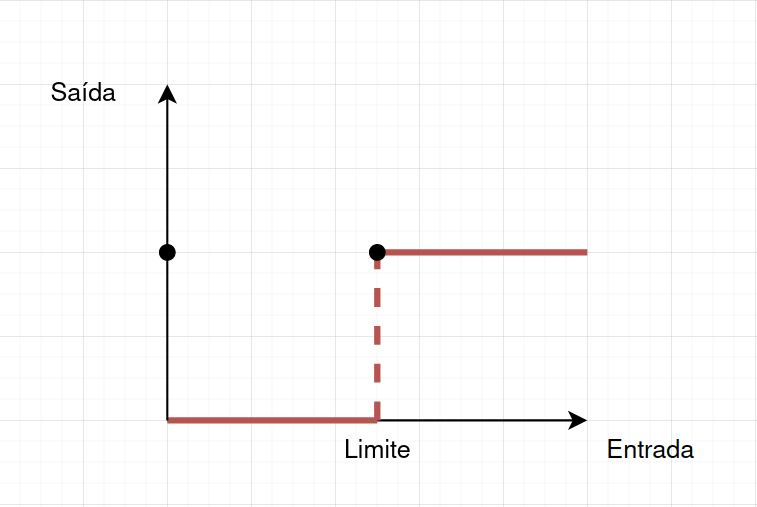
\includegraphics[scale=0.4]{figs/activation_function}
\caption{Função de ativação }\label{ativaçãoF}
\end{figure}


\begin{figure}[H]
\centering
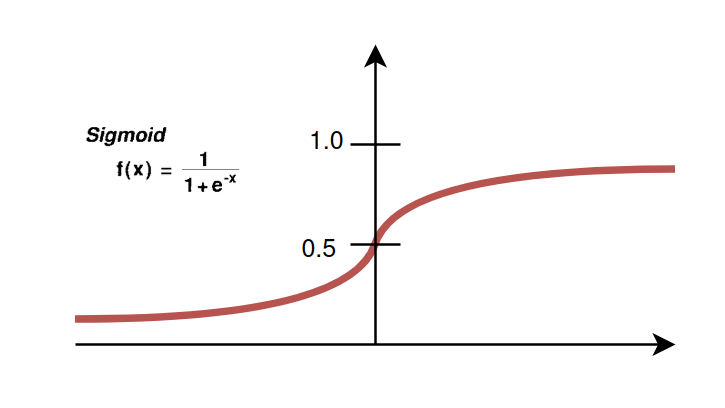
\includegraphics[scale=0.3]{figs/sigmoid}
\caption{Função sigmoide }\label{sigmoidF}
\end{figure}


Tal como nos neurónios biológicos e como é mostrado na fig \ref{node1}, cada neurónio numa rede neural artificial multiplica o valor de entrada por um peso, faz o somatório com outros valores de entrada do mesmo neurónio e por fim processa valor com uma função sigmoide. O valor processado pela função sigmoide torna-se no valor de saída. Cada neurónio poderá ainda ter um número associado chamado de bias, que modifica o valor proveniente do somatório antes de ser processado pela função sigmoide.


\begin{figure}[H]
\centering
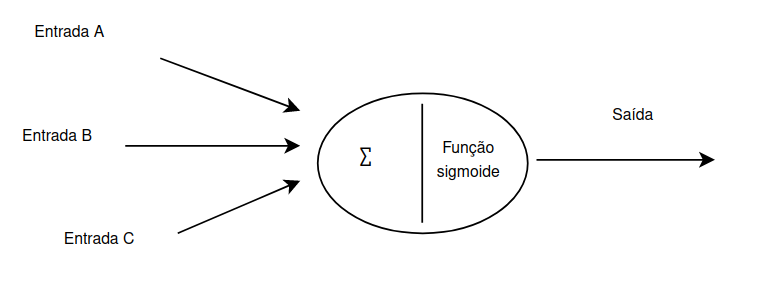
\includegraphics[scale=0.3]{figs/node1.png}
\caption{Entrada e saída de informação em um neurónio} \label{node1}
\end{figure}

Uma rede neural artificial é composta por 3 camadas de neurónios, a camada de entrada que está ligada à camada oculta e que por sua vez está ligada à camada de saída \ref{ANN}. A camada oculta é chamada de caixa negra porque não é possível interpretar como é que a rede neural derivou um determinado resultado. Esta camada poderá ser constituída por uma ou mais camadas de neurónios (colunas de neurónios) interligados entre si.

\begin{figure}[H]
\centering
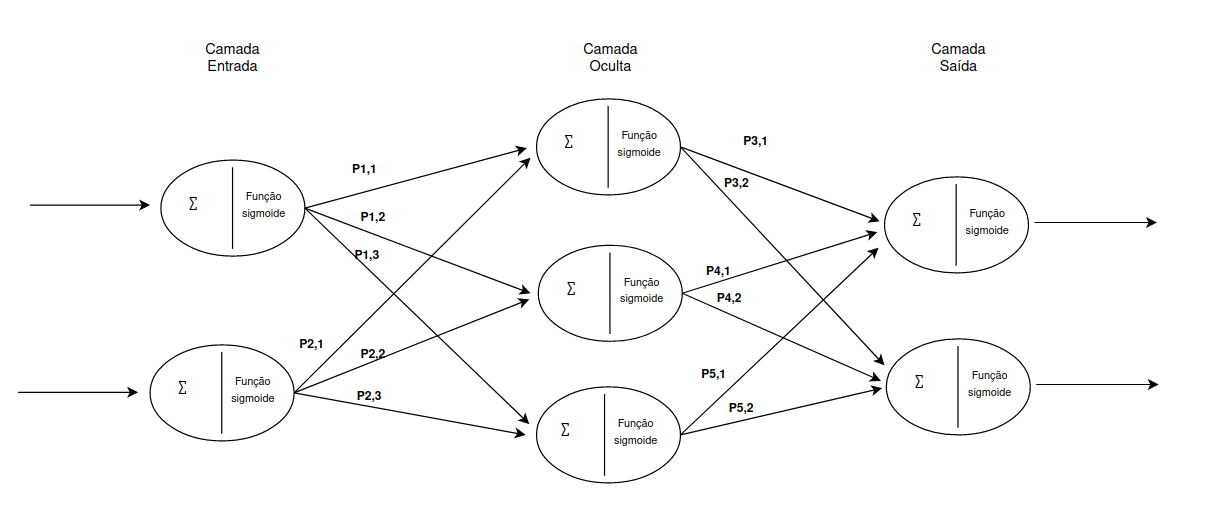
\includegraphics[scale=0.42]{figs/redeNeuralDraw}
\caption{Estrutura de uma Rede Neural}\label{ANN}
\end{figure}



Numa rede neural artificial cada conexão entre neurónios artificiais tem um peso associado. Um valor de peso mais baixo enfraquece o sinal, e um valor de peso mais elevado fortalece o sinal. O processo de aprendizagem consiste no ajustamento destes pesos e, caso tenha, do valor de bias associado a cada neurónio por parte da rede com intuito de melhorar a sua performance. Caso um peso tenha valor 0, o sinal não é transmitido e a rede não pode ser influenciada. A atualização dos pesos é determinada pelo erro entre o valor de saída previsto e o valor correto. O erro é dividido pela proporção dos pesos nas conexões, e o os erros divididos são propagados e remontados \ref{propagaçao}. No entanto, numa estrutura hierárquica é difícil de calcular todos os pesos matematicamente. Existem diversas alternativas, umas mais complexas que outras, que não serão aqui descritas, uma delas, como por exemplo, é o método do gradiente (``gradient descent method''). Sem entrar em grandes detalhes, o método do gradiente é uma técnica para encontrar o ponto mais baixo no qual o custo é minimizado numa função de custo, neste caso, a diferença entre o valor previsto e a resposta obtida para um valor arbitrário inicial do peso P. O modelo pode iniciar com qualquer valor P e alterá-lo gradualmente de modo a que o seu custo seja reduzido e alcance um mínimo. Este é o processo de aprendizagem de uma rede neural artificial.


\begin{figure}[H]
\centering
\includegraphics[scale=0.42]{figs/propagação}
\caption{Propagação dos erros para atualização dos pesos}\label{propagaçao}
\end{figure}




O ``deep'' em ``deep learning'' apenas se refere à profundidade da rede neural, isto é, ao numero de camadas que contém. Uma rede neural que contém mais que 3 camadas, com as de entrada e saída inclusive, pode ser considerada um algoritmo de \ac{dl} ou uma rede neural profunda (``Deep Neural Network''). Uma rede neural com apenas 2 ou 3 camadas é considerada uma rede neural básica.